\section{Planetary Positions}\label{s:ephemeris}

Assuming that the Sun is the central inertial reference point, it is
possible to obtain the position of Earth and all the other planets at any point in time using 
well documented orbital elements of our solar system. This formulation
follows the derivation by JPL and can be found at \cite{JPL}.

\subsection{Julian Day}
In order to obtain the position of the planets, the Julian Day must be
obtained. The Julian Day of January 1st, 2019 is 2,458,485. The Julian
Day of January 1st, 2000 (which is the day of the last inertial frame
update) is 2,451,545. In order to obtain the Julian Day of the current
day, you simply need to count the number of calendar days from January
1st of 2000. Again I have listed the Julian day of January 1st, 2019
to help with this calculation. To compute the orbital elements of the
Earth you must then compute the number of centuries from January 1st,
2000 which is given by the equation below where J is the Julian day
and C is the number of centuries since 1/1/2000. 
\begin{equation}
  C = (J - 2,451,545)/36,525.0
\end{equation}

\subsection{Orbital Elements}
This number is then used in the equations below to obtain the current
semi-major axis, eccentricity, inclination, mean longitude, longitude
of perihelion and the longitude of the ascending node
respectively. The subscript $0$ denotes the orbital element in the
year 2000.
\begin{equation}
  \begin{matrix}
    a = (a_0 + \dot{a}C)AU \\
    e = e_0 + \dot{e}C \\
    i = i_0 + \dot{i}C \\
    L = L_0 + \dot{L}C \\
    \bar{w} = \bar{w}_0 + \dot{\bar{w}}C \\
    \Omega = \Omega_0 + \dot{\Omega}C
  \end{matrix}
\end{equation}
The parameters in the equation above for every planet can be found at
\cite{JPL}. Also, The term $AU$ is an astronomical unit which is equal
to 149,597,870,700 meters. For reference though the parameters for
Earth are shown below. Just in case you are reading this in the not so
distant future, these parameters are only valid until the year
2050 (I may be dead who knows!). Also, the parameters below are for the Earth-Moon barycenter 
which is the center of mass of the Earth and Moon.
\begin{table}[H]
  \begin{center}
  \caption{Orbital Elements of Earth-Moon Barycenter}
\begin{tabular}{cccccc}
    a  &  e  & i & L & long.peri. ($\bar{w}$) & long.node. ($\Omega$)  \\
    \hline
    AU, AU/Cy &  rad, rad/Cy & deg, deg/Cy &  deg, deg/Cy & deg, deg/Cy &  deg, deg/Cy \\
    \hline 
    \hline 
    1.00000261 &  0.01671123  &  -0.00001531 &  100.46457166 &  102.93768193 &  0.0\\
    0.00000562 &  -0.00004392 &  -0.01294668 &   35999.37244981 &  0.32327364  &    0.0\\
    \hline
\end{tabular}
\end{center}
\end{table}
In the table, the first row is the value in the year 2000 and
the second row is the rate per century (Cy). Using these parameters,
compute the argument of the perihelion $w = \bar{w} - \Omega$ and the
mean anomaly $M = L - \bar{w}$. Note that for planets Jupiter, Saturn,
Uranus and Neptune, the mean anomaly has a different form. Basically
anything past the asteroid belt. With the mean anomaly compute you
must modulus this value such that M is between plus or minus 180
degrees. Once that's done you must solve for the eccentric anomaly (E)
using the Kepler equation below where $e^*$ is the eccentricity in
degrees $e^* = 180e/\pi$. 
\begin{equation}
  M = E-e^*sin(E)
\end{equation}
Solving this numerically is pretty simple and only requires a few
iterations of the loop below using the C++ programming language. This
loop can easily be adapted to any language on modern computers. C++ is
shown here in the event this is used for embedded processors in future
satellite systems. 
\begin{verbatim}
  E = M + e*180.0/PI*sin(M*PI/180.0);
  dM = 1;
  dE = 0;
  while (abs(dM) > 1e-6) {
    dM = M - (E - e*180.0/PI*sin(E*PI/180.0));
    dE = dM/(1.0-e*cos(E*PI/180.0));
    E += dE;
  }        
\end{verbatim}
\subsection{Sun Centered Inertial Coordinates}
At this point the spatial coordinates can be obtained in the planet's
orbital plane where the semi-latus rectum or sometimes simply called
the parameter is $p=a(1-e)$. 
\begin{equation}
  \begin{Bmatrix} x' \\ y' \\ z' \end{Bmatrix} = \begin{Bmatrix} a(cos(\pi E/180) - e)
    \\ a\sqrt{1-e^2}sin(\pi E/180) \\ 0 \end{Bmatrix}
\end{equation}
Notice that the value $z'$ is zero. This is because orbits are all two
dimensional. In order to obtain the coordinates of the planet in the
J2000 ecliptic plane, the equation below is used which is similar to
the standard Euler angle transformation matrix only the 3-1-3 rotation
sequence is used rather than 3-2-1. 
\begin{equation}
  \begin{Bmatrix} x \\ y \\ z \end{Bmatrix}_{J2000} = \begin{bmatrix} c_wc_{\Omega}-s_ws_{\Omega}c_i &
    -s_wc_{\Omega}-c_ws_{\Omega}c_i & 0
    \\ c_ws_{\Omega}+s_wc_{\Omega}c_i &
    -s_ws_{\Omega}+c_wc_{\Omega}c_i & 0 \\
    s_ws_i & c_ws_i & 0 \end{bmatrix} \begin{Bmatrix} x' \\ y' \\ z' \end{Bmatrix}
\end{equation}
Running through this formulation for all the planets in the Solar
System including Pluto it is possible to plot the position of all
planets. The figures below are for January 1st, 2019.
\begin{figure}[H]
  \begin{center}
  \begin{tabular}{cc}
  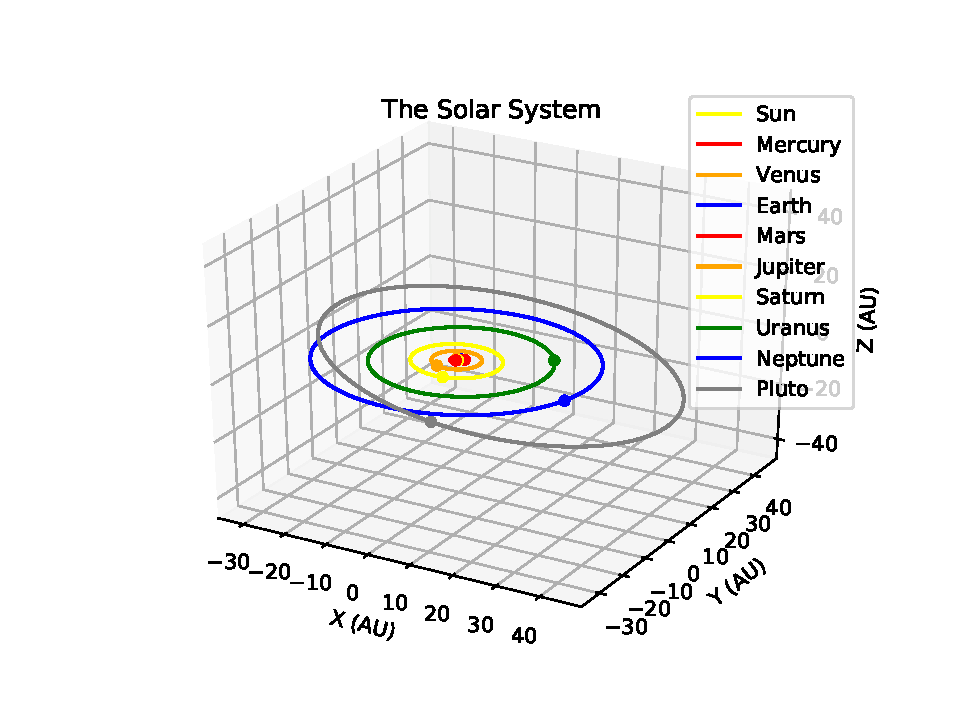
\includegraphics[height=70mm, width=80mm]{Figures/all_planets_isometric.pdf}&
  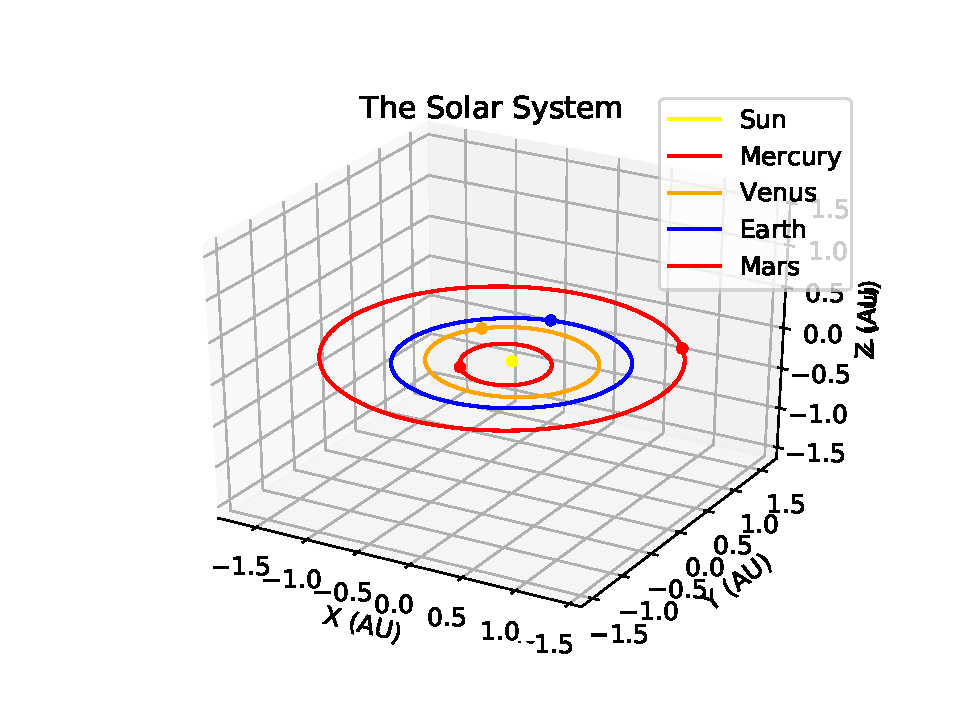
\includegraphics[height=70mm, width=80mm]{Figures/inner_planets_isometric.pdf}\\
  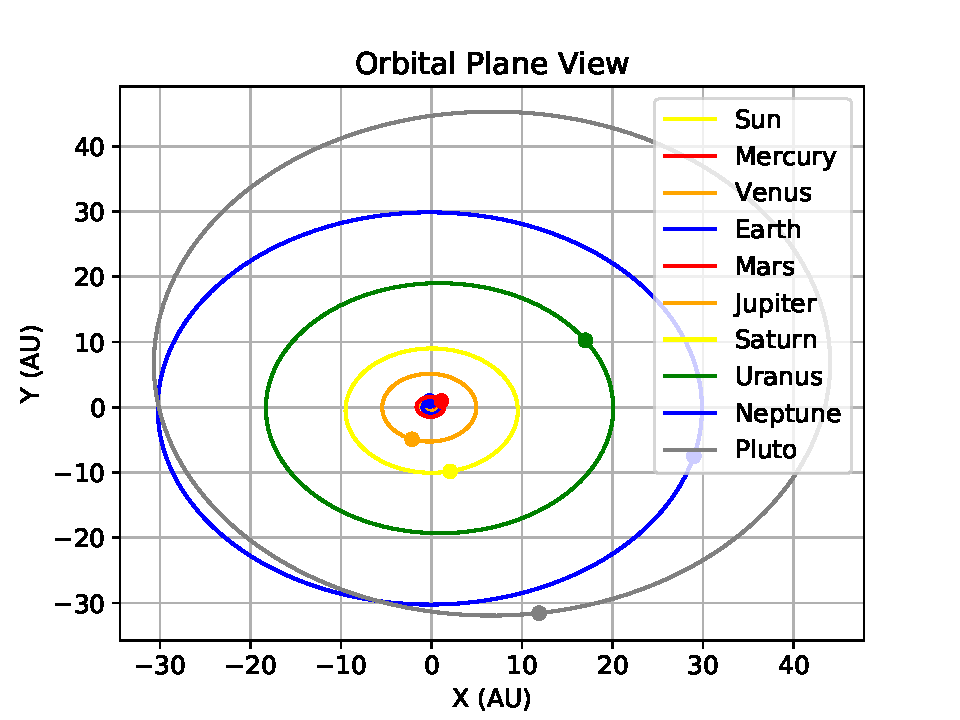
\includegraphics[height=70mm, width=80mm]{Figures/top_down_view_all_planets.pdf}&
  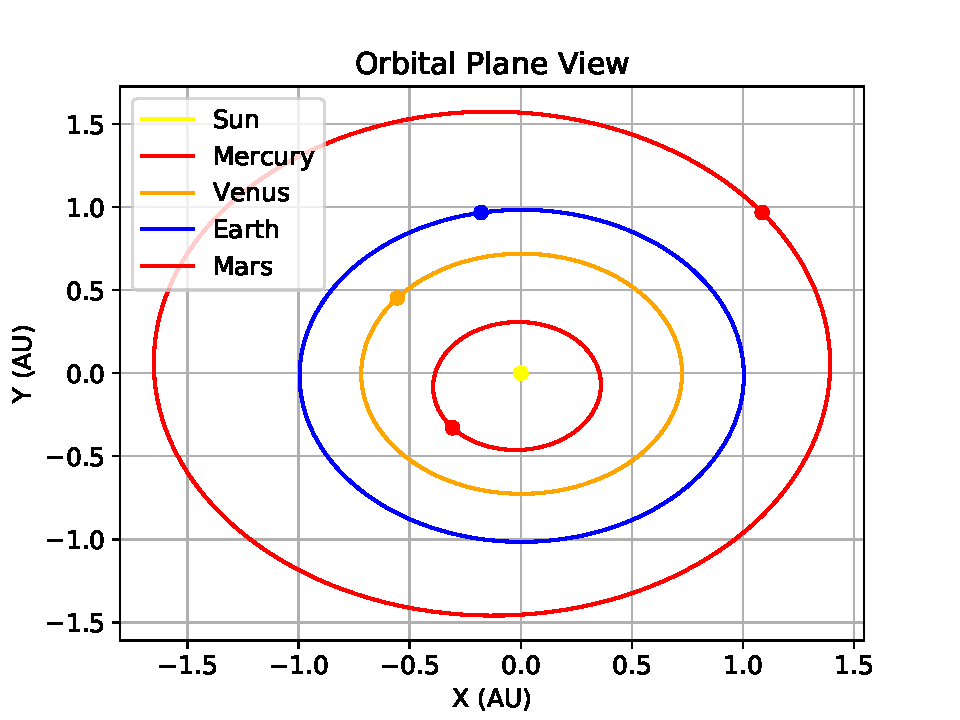
\includegraphics[height=70mm, width=80mm]{Figures/inner_planets_top_down.pdf}\\
  \end{tabular}
  \end{center}
  \caption{Position of Planets using Orbital Elements}
\end{figure}
